\chapter{Implementación\label{cap:implementacion}}

TODO: [Introducción]


\section{Back-End\label{sec:imp:back_end}}

Introducción implementación back-end

Stack de librerías: io.js, express, supervisor, apiDoc

1 párrafo: servicio instalado que se autoinicia

\begin{figure}[!htp]
  \centering
  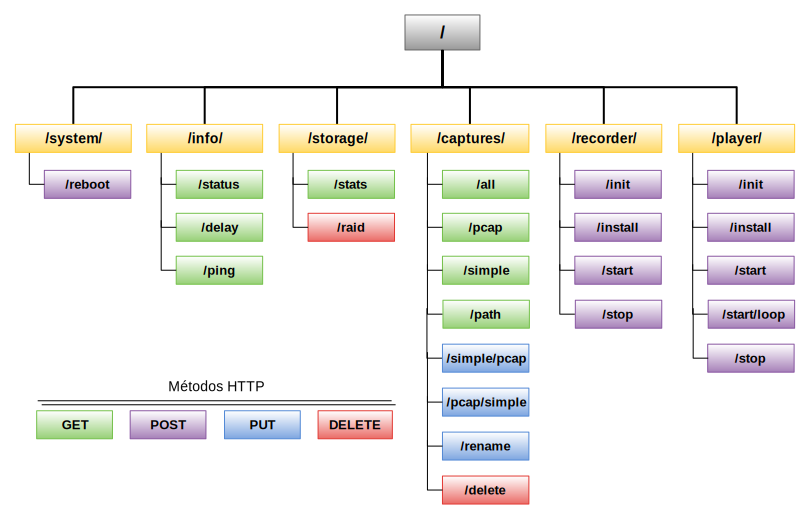
\includegraphics[width=\textwidth,clip=true]{arbol_metodos}
  \caption{Métodos públicos del \gls{servicioweb} \gls{FPGA}.}
  \label{fig:arbol_metodos}
\end{figure}

Arbol rutas \ref{fig:fpga_estado}

\begin{figure}[!htp]
  \centering
  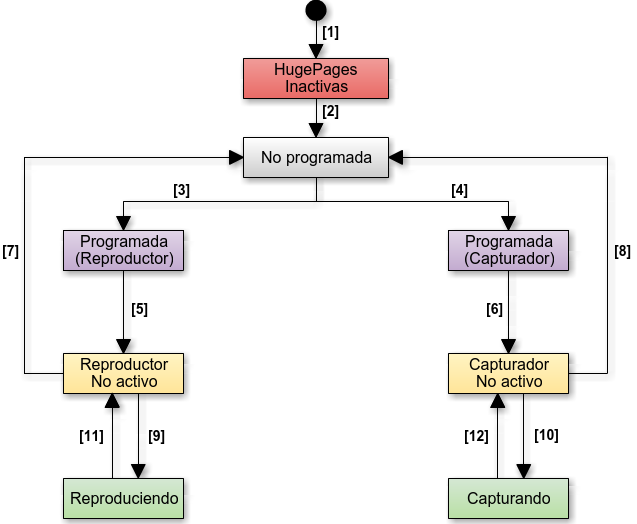
\includegraphics[width=\textwidth,clip=true]{fpga_estado}
  \caption{Máquina de Estados Finita para el estado de la \gls{FPGA}.}
  \label{fig:fpga_estado}
\end{figure}

FSM de estados FPGA \ref{fig:fpga_estado}

Captura árbol de archivos \ref{fig:arbol_codigo}

\begin{figure}[!htp]
  \begin{center}
    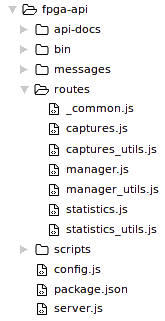
\includegraphics[width=0.3\textwidth,clip=true]{capturas/arbol_backend}
    \hspace{1cm}
    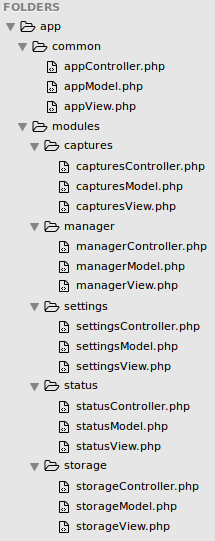
\includegraphics[width=0.3\textwidth,clip=true]{capturas/arbol_frontend}
  \caption{Árboles con los principales archivos de código del \gls{back-end} (a la izquierda) y del \gls{front-end} (a la derecha).}
  \label{fig:arbol_codigo}
  \end{center}
\end{figure}

Captura wiki


\section{Front-End\label{sec:imp:front_end}}

Introducción

Resultado Capturas diseño responsive (misma página desde dos sitios)

Stack de librerías: MVC propio,Bootstrap,jQuery,gettext, etc.

Captura árbol de archivos \ref{fig:arbol_codigo}

Internacionalización

Temas (captura algún temas)

\section{Documentación\label{sec:imp:docs}}

Captura documentación online backend y front-end